\documentclass[11pt,compress,t,notes=noshow, xcolor=table]{beamer}
\usepackage[]{graphicx}\usepackage[]{color}
% maxwidth is the original width if it is less than linewidth
% otherwise use linewidth (to make sure the graphics do not exceed the margin)
\makeatletter
\def\maxwidth{ %
  \ifdim\Gin@nat@width>\linewidth
    \linewidth
  \else
    \Gin@nat@width
  \fi
}
\makeatother

\definecolor{fgcolor}{rgb}{0.345, 0.345, 0.345}
\newcommand{\hlnum}[1]{\textcolor[rgb]{0.686,0.059,0.569}{#1}}%
\newcommand{\hlstr}[1]{\textcolor[rgb]{0.192,0.494,0.8}{#1}}%
\newcommand{\hlcom}[1]{\textcolor[rgb]{0.678,0.584,0.686}{\textit{#1}}}%
\newcommand{\hlopt}[1]{\textcolor[rgb]{0,0,0}{#1}}%
\newcommand{\hlstd}[1]{\textcolor[rgb]{0.345,0.345,0.345}{#1}}%
\newcommand{\hlkwa}[1]{\textcolor[rgb]{0.161,0.373,0.58}{\textbf{#1}}}%
\newcommand{\hlkwb}[1]{\textcolor[rgb]{0.69,0.353,0.396}{#1}}%
\newcommand{\hlkwc}[1]{\textcolor[rgb]{0.333,0.667,0.333}{#1}}%
\newcommand{\hlkwd}[1]{\textcolor[rgb]{0.737,0.353,0.396}{\textbf{#1}}}%
\let\hlipl\hlkwb

\usepackage{framed}
\makeatletter
\newenvironment{kframe}{%
 \def\at@end@of@kframe{}%
 \ifinner\ifhmode%
  \def\at@end@of@kframe{\end{minipage}}%
  \begin{minipage}{\columnwidth}%
 \fi\fi%
 \def\FrameCommand##1{\hskip\@totalleftmargin \hskip-\fboxsep
 \colorbox{shadecolor}{##1}\hskip-\fboxsep
     % There is no \\@totalrightmargin, so:
     \hskip-\linewidth \hskip-\@totalleftmargin \hskip\columnwidth}%
 \MakeFramed {\advance\hsize-\width
   \@totalleftmargin\z@ \linewidth\hsize
   \@setminipage}}%
 {\par\unskip\endMakeFramed%
 \at@end@of@kframe}
\makeatother

\definecolor{shadecolor}{rgb}{.97, .97, .97}
\definecolor{messagecolor}{rgb}{0, 0, 0}
\definecolor{warningcolor}{rgb}{1, 0, 1}
\definecolor{errorcolor}{rgb}{1, 0, 0}
\newenvironment{knitrout}{}{} % an empty environment to be redefined in TeX

\usepackage{alltt}
\newcommand{\SweaveOpts}[1]{}  % do not interfere with LaTeX
\newcommand{\SweaveInput}[1]{} % because they are not real TeX commands
\newcommand{\Sexpr}[1]{}       % will only be parsed by R
\newcommand{\xmark}{\ding{55}}%


\usepackage[english]{babel}
\usepackage[utf8]{inputenc}

\usepackage{dsfont}
\usepackage{verbatim}
\usepackage{amsmath}
\usepackage{amsfonts}
\usepackage{amssymb}
\usepackage{bm}
\usepackage{csquotes}
\usepackage{multirow}
\usepackage{longtable}
\usepackage{booktabs}
\usepackage{enumerate}
\usepackage[absolute,overlay]{textpos}
\usepackage{psfrag}
\usepackage{algorithm}
\usepackage{algpseudocode}
\usepackage{eqnarray}
\usepackage{arydshln}
\usepackage{tabularx}
\usepackage{placeins}
\usepackage{tikz}
\usepackage{setspace}
\usepackage{colortbl}
\usepackage{mathtools}
\usepackage{wrapfig}
\usepackage{bm}
\usepackage{amsmath}
\usepackage{pifont}
\usepackage[round]{natbib}
\usepackage{hyperref}

\usetikzlibrary{shapes,arrows,automata,positioning,calc,chains,trees, shadows}
\tikzset{
  %Define standard arrow tip
  >=stealth',
  %Define style for boxes
  punkt/.style={
    rectangle,
    rounded corners,
    draw=black, very thick,
    text width=6.5em,
    minimum height=2em,
    text centered},
  % Define arrow style
  pil/.style={
    ->,
    thick,
    shorten <=2pt,
    shorten >=2pt,}
}

\usepackage{subfig}

% Defines macros and environments
\usepackage{../../style/lmu-lecture}


\let\code=\texttt
\let\proglang=\textsf

\setkeys{Gin}{width=0.9\textwidth}

\setbeamertemplate{frametitle}{\expandafter\uppercase\expandafter\insertframetitle}

% basic latex stuff
\newcommand{\pkg}[1]{{\fontseries{b}\selectfont #1}} % fontstyle for R packages

% Often used in exercise Rnw files, still relevant?
\newcommand{\lz}{\vspace{0.5cm}} % vertical space
\newcommand{\dlz}{\vspace{1cm}}  % double vertical space

% Unused and about to be deleted
\newcommand{\oneliner}[1] % Oneliner for important statements
{\begin{block}{}\begin{center}\begin{Large}#1\end{Large}\end{center}\end{block}}


%--------------------%
%  New environments  %
%--------------------%

 % Frame with breaks and verbatim // this is used very often
\newenvironment{vbframe}
{
\begin{frame}[containsverbatim,allowframebreaks]
}
{
\end{frame}
}

% Frame with verbatim without breaks (to avoid numbering one slided frames)
% This is not used anywhere but I can see it being useful
\newenvironment{vframe}
{
\begin{frame}[containsverbatim]
}
{
\end{frame}
}

% Itemize block
\newenvironment{blocki}[1]
{
\begin{block}{#1}\begin{itemize}
}
{
\end{itemize}\end{block}
}

%--------------%
%  Citebutton  %
%--------------%
% Example usage (from slides-cart-discussion.tex)
% \citebutton{Breiman, 1984}{https://www.taylorfrancis.com/books/mono/10.1201/9781315139470/classification-regression-trees-leo-breiman}
\newcommand{\citebutton}[2]{%
\NoCaseChange{\resizebox{!}{9pt}{\protect\beamergotobutton{\href{#2}{#1}}}}%
}

% textcolor that works in mathmode
% https://tex.stackexchange.com/a/261480
% Used e.g. in forests/slides-forests-bagging.tex
% [...] \textcolor{blue}{\tfrac{1}{M}\sum^M_{m} [...]
\makeatletter
\renewcommand*{\@textcolor}[3]{%
  \protect\leavevmode
  \begingroup
    \color#1{#2}#3%
  \endgroup
}
\makeatother





% dependencies: amsmath, amssymb, dsfont
% math spaces
\ifdefined\N
\renewcommand{\N}{\mathds{N}} % N, naturals
\else \newcommand{\N}{\mathds{N}} \fi
\newcommand{\Z}{\mathds{Z}} % Z, integers
\newcommand{\Q}{\mathds{Q}} % Q, rationals
\newcommand{\R}{\mathds{R}} % R, reals
\ifdefined\C
\renewcommand{\C}{\mathds{C}} % C, complex
\else \newcommand{\C}{\mathds{C}} \fi
\newcommand{\continuous}{\mathcal{C}} % C, space of continuous functions
\newcommand{\M}{\mathcal{M}} % machine numbers
\newcommand{\epsm}{\epsilon_m} % maximum error

% counting / finite sets
\newcommand{\setzo}{\{0, 1\}} % set 0, 1
\newcommand{\setmp}{\{-1, +1\}} % set -1, 1
\newcommand{\unitint}{[0, 1]} % unit interval

% basic math stuff
\newcommand{\xt}{\tilde x} % x tilde
\DeclareMathOperator*{\argmax}{arg\,max} % argmax
\DeclareMathOperator*{\argmin}{arg\,min} % argmin
\newcommand{\argminlim}{\mathop{\mathrm{arg\,min}}\limits} % argmax with limits
\newcommand{\argmaxlim}{\mathop{\mathrm{arg\,max}}\limits} % argmin with limits
\newcommand{\sign}{\operatorname{sign}} % sign, signum
\newcommand{\I}{\mathbb{I}} % I, indicator
\newcommand{\order}{\mathcal{O}} % O, order
\newcommand{\bigO}{\mathcal{O}} % Big-O Landau
\newcommand{\littleo}{{o}} % Little-o Landau
\newcommand{\pd}[2]{\frac{\partial{#1}}{\partial #2}} % partial derivative
\newcommand{\floorlr}[1]{\left\lfloor #1 \right\rfloor} % floor
\newcommand{\ceillr}[1]{\left\lceil #1 \right\rceil} % ceiling
\newcommand{\indep}{\perp \!\!\! \perp} % independence symbol

% sums and products
\newcommand{\sumin}{\sum\limits_{i=1}^n} % summation from i=1 to n
\newcommand{\sumim}{\sum\limits_{i=1}^m} % summation from i=1 to m
\newcommand{\sumjn}{\sum\limits_{j=1}^n} % summation from j=1 to p
\newcommand{\sumjp}{\sum\limits_{j=1}^p} % summation from j=1 to p
\newcommand{\sumik}{\sum\limits_{i=1}^k} % summation from i=1 to k
\newcommand{\sumkg}{\sum\limits_{k=1}^g} % summation from k=1 to g
\newcommand{\sumjg}{\sum\limits_{j=1}^g} % summation from j=1 to g
\newcommand{\meanin}{\frac{1}{n} \sum\limits_{i=1}^n} % mean from i=1 to n
\newcommand{\meanim}{\frac{1}{m} \sum\limits_{i=1}^m} % mean from i=1 to n
\newcommand{\meankg}{\frac{1}{g} \sum\limits_{k=1}^g} % mean from k=1 to g
\newcommand{\prodin}{\prod\limits_{i=1}^n} % product from i=1 to n
\newcommand{\prodkg}{\prod\limits_{k=1}^g} % product from k=1 to g
\newcommand{\prodjp}{\prod\limits_{j=1}^p} % product from j=1 to p

% linear algebra
\newcommand{\one}{\bm{1}} % 1, unitvector
\newcommand{\zero}{\mathbf{0}} % 0-vector
\newcommand{\id}{\bm{I}} % I, identity
\newcommand{\diag}{\operatorname{diag}} % diag, diagonal
\newcommand{\trace}{\operatorname{tr}} % tr, trace
\newcommand{\spn}{\operatorname{span}} % span
\newcommand{\scp}[2]{\left\langle #1, #2 \right\rangle} % <.,.>, scalarproduct
\newcommand{\mat}[1]{\begin{pmatrix} #1 \end{pmatrix}} % short pmatrix command
\newcommand{\Amat}{\mathbf{A}} % matrix A
\newcommand{\Deltab}{\mathbf{\Delta}} % error term for vectors

% basic probability + stats
\renewcommand{\P}{\mathds{P}} % P, probability
\newcommand{\E}{\mathds{E}} % E, expectation
\newcommand{\var}{\mathsf{Var}} % Var, variance
\newcommand{\cov}{\mathsf{Cov}} % Cov, covariance
\newcommand{\corr}{\mathsf{Corr}} % Corr, correlation
\newcommand{\normal}{\mathcal{N}} % N of the normal distribution
\newcommand{\iid}{\overset{i.i.d}{\sim}} % dist with i.i.d superscript
\newcommand{\distas}[1]{\overset{#1}{\sim}} % ... is distributed as ...

% machine learning
\newcommand{\Xspace}{\mathcal{X}} % X, input space
\newcommand{\Yspace}{\mathcal{Y}} % Y, output space
\newcommand{\Zspace}{\mathcal{Z}} % Z, space of sampled datapoints
\newcommand{\nset}{\{1, \ldots, n\}} % set from 1 to n
\newcommand{\pset}{\{1, \ldots, p\}} % set from 1 to p
\newcommand{\gset}{\{1, \ldots, g\}} % set from 1 to g
\newcommand{\Pxy}{\mathbb{P}_{xy}} % P_xy
\newcommand{\Exy}{\mathbb{E}_{xy}} % E_xy: Expectation over random variables xy
\newcommand{\xv}{\mathbf{x}} % vector x (bold)
\newcommand{\xtil}{\tilde{\mathbf{x}}} % vector x-tilde (bold)
\newcommand{\yv}{\mathbf{y}} % vector y (bold)
\newcommand{\xy}{(\xv, y)} % observation (x, y)
\newcommand{\xvec}{\left(x_1, \ldots, x_p\right)^\top} % (x1, ..., xp)
\newcommand{\Xmat}{\mathbf{X}} % Design matrix
\newcommand{\allDatasets}{\mathds{D}} % The set of all datasets
\newcommand{\allDatasetsn}{\mathds{D}_n}  % The set of all datasets of size n
\newcommand{\D}{\mathcal{D}} % D, data
\newcommand{\Dn}{\D_n} % D_n, data of size n
\newcommand{\Dtrain}{\mathcal{D}_{\text{train}}} % D_train, training set
\newcommand{\Dtest}{\mathcal{D}_{\text{test}}} % D_test, test set
\newcommand{\xyi}[1][i]{\left(\xv^{(#1)}, y^{(#1)}\right)} % (x^i, y^i), i-th observation
\newcommand{\Dset}{\left( \xyi[1], \ldots, \xyi[n]\right)} % {(x1,y1)), ..., (xn,yn)}, data
\newcommand{\defAllDatasetsn}{(\Xspace \times \Yspace)^n} % Def. of the set of all datasets of size n
\newcommand{\defAllDatasets}{\bigcup_{n \in \N}(\Xspace \times \Yspace)^n} % Def. of the set of all datasets
\newcommand{\xdat}{\left\{ \xv^{(1)}, \ldots, \xv^{(n)}\right\}} % {x1, ..., xn}, input data
\newcommand{\ydat}{\left\{ \yv^{(1)}, \ldots, \yv^{(n)}\right\}} % {y1, ..., yn}, input data
\newcommand{\yvec}{\left(y^{(1)}, \hdots, y^{(n)}\right)^\top} % (y1, ..., yn), vector of outcomes
\newcommand{\greekxi}{\xi} % Greek letter xi
\renewcommand{\xi}[1][i]{\xv^{(#1)}} % x^i, i-th observed value of x
\newcommand{\yi}[1][i]{y^{(#1)}} % y^i, i-th observed value of y
\newcommand{\xivec}{\left(x^{(i)}_1, \ldots, x^{(i)}_p\right)^\top} % (x1^i, ..., xp^i), i-th observation vector
\newcommand{\xj}{\xv_j} % x_j, j-th feature
\newcommand{\xjvec}{\left(x^{(1)}_j, \ldots, x^{(n)}_j\right)^\top} % (x^1_j, ..., x^n_j), j-th feature vector
\newcommand{\phiv}{\mathbf{\phi}} % Basis transformation function phi
\newcommand{\phixi}{\mathbf{\phi}^{(i)}} % Basis transformation of xi: phi^i := phi(xi)

%%%%%% ml - models general
\newcommand{\lamv}{\bm{\lambda}} % lambda vector, hyperconfiguration vector
\newcommand{\Lam}{\bm{\Lambda}}	 % Lambda, space of all hpos
% Inducer / Inducing algorithm
\newcommand{\preimageInducer}{\left(\defAllDatasets\right)\times\Lam} % Set of all datasets times the hyperparameter space
\newcommand{\preimageInducerShort}{\allDatasets\times\Lam} % Set of all datasets times the hyperparameter space
% Inducer / Inducing algorithm
\newcommand{\ind}{\mathcal{I}} % Inducer, inducing algorithm, learning algorithm

% continuous prediction function f
\newcommand{\ftrue}{f_{\text{true}}}  % True underlying function (if a statistical model is assumed)
\newcommand{\ftruex}{\ftrue(\xv)} % True underlying function (if a statistical model is assumed)
\newcommand{\fx}{f(\xv)} % f(x), continuous prediction function
\newcommand{\fdomains}{f: \Xspace \rightarrow \R^g} % f with domain and co-domain
\newcommand{\Hspace}{\mathcal{H}} % hypothesis space where f is from
\newcommand{\fbayes}{f^{\ast}} % Bayes-optimal model
\newcommand{\fxbayes}{f^{\ast}(\xv)} % Bayes-optimal model
\newcommand{\fkx}[1][k]{f_{#1}(\xv)} % f_j(x), discriminant component function
\newcommand{\fh}{\hat{f}} % f hat, estimated prediction function
\newcommand{\fxh}{\fh(\xv)} % fhat(x)
\newcommand{\fxt}{f(\xv ~|~ \thetav)} % f(x | theta)
\newcommand{\fxi}{f\left(\xv^{(i)}\right)} % f(x^(i))
\newcommand{\fxih}{\hat{f}\left(\xv^{(i)}\right)} % f(x^(i))
\newcommand{\fxit}{f\left(\xv^{(i)} ~|~ \thetav\right)} % f(x^(i) | theta)
\newcommand{\fhD}{\fh_{\D}} % fhat_D, estimate of f based on D
\newcommand{\fhDtrain}{\fh_{\Dtrain}} % fhat_Dtrain, estimate of f based on D
\newcommand{\fhDnlam}{\fh_{\Dn, \lamv}} %model learned on Dn with hp lambda
\newcommand{\fhDlam}{\fh_{\D, \lamv}} %model learned on D with hp lambda
\newcommand{\fhDnlams}{\fh_{\Dn, \lamv^\ast}} %model learned on Dn with optimal hp lambda
\newcommand{\fhDlams}{\fh_{\D, \lamv^\ast}} %model learned on D with optimal hp lambda

% discrete prediction function h
\newcommand{\hx}{h(\xv)} % h(x), discrete prediction function
\newcommand{\hh}{\hat{h}} % h hat
\newcommand{\hxh}{\hat{h}(\xv)} % hhat(x)
\newcommand{\hxt}{h(\xv | \thetav)} % h(x | theta)
\newcommand{\hxi}{h\left(\xi\right)} % h(x^(i))
\newcommand{\hxit}{h\left(\xi ~|~ \thetav\right)} % h(x^(i) | theta)
\newcommand{\hbayes}{h^{\ast}} % Bayes-optimal classification model
\newcommand{\hxbayes}{h^{\ast}(\xv)} % Bayes-optimal classification model

% yhat
\newcommand{\yh}{\hat{y}} % yhat for prediction of target
\newcommand{\yih}{\hat{y}^{(i)}} % yhat^(i) for prediction of ith targiet
\newcommand{\resi}{\yi- \yih}

% theta
\newcommand{\thetah}{\hat{\theta}} % theta hat
\newcommand{\thetav}{\bm{\theta}} % theta vector
\newcommand{\thetavh}{\bm{\hat\theta}} % theta vector hat
\newcommand{\thetat}[1][t]{\thetav^{[#1]}} % theta^[t] in optimization
\newcommand{\thetatn}[1][t]{\thetav^{[#1 +1]}} % theta^[t+1] in optimization
\newcommand{\thetahDnlam}{\thetavh_{\Dn, \lamv}} %theta learned on Dn with hp lambda
\newcommand{\thetahDlam}{\thetavh_{\D, \lamv}} %theta learned on D with hp lambda
\newcommand{\mint}{\min_{\thetav \in \Theta}} % min problem theta
\newcommand{\argmint}{\argmin_{\thetav \in \Theta}} % argmin theta

% densities + probabilities
% pdf of x
\newcommand{\pdf}{p} % p
\newcommand{\pdfx}{p(\xv)} % p(x)
\newcommand{\pixt}{\pi(\xv~|~ \thetav)} % pi(x|theta), pdf of x given theta
\newcommand{\pixit}[1][i]{\pi\left(\xi[#1] ~|~ \thetav\right)} % pi(x^i|theta), pdf of x given theta
\newcommand{\pixii}[1][i]{\pi\left(\xi[#1]\right)} % pi(x^i), pdf of i-th x

% pdf of (x, y)
\newcommand{\pdfxy}{p(\xv,y)} % p(x, y)
\newcommand{\pdfxyt}{p(\xv, y ~|~ \thetav)} % p(x, y | theta)
\newcommand{\pdfxyit}{p\left(\xi, \yi ~|~ \thetav\right)} % p(x^(i), y^(i) | theta)

% pdf of x given y
\newcommand{\pdfxyk}[1][k]{p(\xv | y= #1)} % p(x | y = k)
\newcommand{\lpdfxyk}[1][k]{\log p(\xv | y= #1)} % log p(x | y = k)
\newcommand{\pdfxiyk}[1][k]{p\left(\xi | y= #1 \right)} % p(x^i | y = k)

% prior probabilities
\newcommand{\pik}[1][k]{\pi_{#1}} % pi_k, prior
\newcommand{\lpik}[1][k]{\log \pi_{#1}} % log pi_k, log of the prior
\newcommand{\pit}{\pi(\thetav)} % Prior probability of parameter theta

% posterior probabilities
\newcommand{\post}{\P(y = 1 ~|~ \xv)} % P(y = 1 | x), post. prob for y=1
\newcommand{\postk}[1][k]{\P(y = #1 ~|~ \xv)} % P(y = k | y), post. prob for y=k
\newcommand{\pidomains}{\pi: \Xspace \rightarrow \unitint} % pi with domain and co-domain
\newcommand{\pibayes}{\pi^{\ast}} % Bayes-optimal classification model
\newcommand{\pixbayes}{\pi^{\ast}(\xv)} % Bayes-optimal classification model
\newcommand{\pix}{\pi(\xv)} % pi(x), P(y = 1 | x)
\newcommand{\piv}{\bm{\pi}} % pi, bold, as vector
\newcommand{\pikx}[1][k]{\pi_{#1}(\xv)} % pi_k(x), P(y = k | x)
\newcommand{\pikxt}[1][k]{\pi_{#1}(\xv ~|~ \thetav)} % pi_k(x | theta), P(y = k | x, theta)
\newcommand{\pixh}{\hat \pi(\xv)} % pi(x) hat, P(y = 1 | x) hat
\newcommand{\pikxh}[1][k]{\hat \pi_{#1}(\xv)} % pi_k(x) hat, P(y = k | x) hat
\newcommand{\pixih}{\hat \pi(\xi)} % pi(x^(i)) with hat
\newcommand{\pikxih}[1][k]{\hat \pi_{#1}(\xi)} % pi_k(x^(i)) with hat
\newcommand{\pdfygxt}{p(y ~|~\xv, \thetav)} % p(y | x, theta)
\newcommand{\pdfyigxit}{p\left(\yi ~|~\xi, \thetav\right)} % p(y^i |x^i, theta)
\newcommand{\lpdfygxt}{\log \pdfygxt } % log p(y | x, theta)
\newcommand{\lpdfyigxit}{\log \pdfyigxit} % log p(y^i |x^i, theta)

% probababilistic
\newcommand{\bayesrulek}[1][k]{\frac{\P(\xv | y= #1) \P(y= #1)}{\P(\xv)}} % Bayes rule
\newcommand{\muk}{\bm{\mu_k}} % mean vector of class-k Gaussian (discr analysis)

% residual and margin
\newcommand{\eps}{\epsilon} % residual, stochastic
\newcommand{\epsv}{\bm{\epsilon}} % residual, stochastic, as vector
\newcommand{\epsi}{\epsilon^{(i)}} % epsilon^i, residual, stochastic
\newcommand{\epsh}{\hat{\epsilon}} % residual, estimated
\newcommand{\epsvh}{\hat{\epsv}} % residual, estimated, vector
\newcommand{\yf}{y \fx} % y f(x), margin
\newcommand{\yfi}{\yi \fxi} % y^i f(x^i), margin
\newcommand{\Sigmah}{\hat \Sigma} % estimated covariance matrix
\newcommand{\Sigmahj}{\hat \Sigma_j} % estimated covariance matrix for the j-th class

% ml - loss, risk, likelihood
\newcommand{\Lyf}{L\left(y, f\right)} % L(y, f), loss function
\newcommand{\Lypi}{L\left(y, \pi\right)} % L(y, pi), loss function
\newcommand{\Lxy}{L\left(y, \fx\right)} % L(y, f(x)), loss function
\newcommand{\Lxyi}{L\left(\yi, \fxi\right)} % loss of observation
\newcommand{\Lxyt}{L\left(y, \fxt\right)} % loss with f parameterized
\newcommand{\Lxyit}{L\left(\yi, \fxit\right)} % loss of observation with f parameterized
\newcommand{\Lxym}{L\left(\yi, f\left(\bm{\tilde{x}}^{(i)} ~|~ \thetav\right)\right)} % loss of observation with f parameterized
\newcommand{\Lpixy}{L\left(y, \pix\right)} % loss in classification
\newcommand{\Lpiv}{L\left(y, \piv\right)} % loss in classification
\newcommand{\Lpixyi}{L\left(\yi, \pixii\right)} % loss of observation in classification
\newcommand{\Lpixyt}{L\left(y, \pixt\right)} % loss with pi parameterized
\newcommand{\Lpixyit}{L\left(\yi, \pixit\right)} % loss of observation with pi parameterized
\newcommand{\Lhxy}{L\left(y, \hx\right)} % L(y, h(x)), loss function on discrete classes
\newcommand{\Lr}{L\left(r\right)} % L(r), loss defined on residual (reg) / margin (classif)
\newcommand{\lone}{|y - \fx|} % L1 loss
\newcommand{\ltwo}{\left(y - \fx\right)^2} % L2 loss
\newcommand{\lbernoullimp}{\ln(1 + \exp(-y \cdot \fx))} % Bernoulli loss for -1, +1 encoding
\newcommand{\lbernoullizo}{- y \cdot \fx + \log(1 + \exp(\fx))} % Bernoulli loss for 0, 1 encoding
\newcommand{\lcrossent}{- y \log \left(\pix\right) - (1 - y) \log \left(1 - \pix\right)} % cross-entropy loss
\newcommand{\lbrier}{\left(\pix - y \right)^2} % Brier score
\newcommand{\risk}{\mathcal{R}} % R, risk
\newcommand{\riskbayes}{\mathcal{R}^\ast}
\newcommand{\riskf}{\risk(f)} % R(f), risk
\newcommand{\riskdef}{\E_{y|\xv}\left(\Lxy \right)} % risk def (expected loss)
\newcommand{\riskt}{\mathcal{R}(\thetav)} % R(theta), risk
\newcommand{\riske}{\mathcal{R}_{\text{emp}}} % R_emp, empirical risk w/o factor 1 / n
\newcommand{\riskeb}{\bar{\mathcal{R}}_{\text{emp}}} % R_emp, empirical risk w/ factor 1 / n
\newcommand{\riskef}{\riske(f)} % R_emp(f)
\newcommand{\risket}{\mathcal{R}_{\text{emp}}(\thetav)} % R_emp(theta)
\newcommand{\riskr}{\mathcal{R}_{\text{reg}}} % R_reg, regularized risk
\newcommand{\riskrt}{\mathcal{R}_{\text{reg}}(\thetav)} % R_reg(theta)
\newcommand{\riskrf}{\riskr(f)} % R_reg(f)
\newcommand{\riskrth}{\hat{\mathcal{R}}_{\text{reg}}(\thetav)} % hat R_reg(theta)
\newcommand{\risketh}{\hat{\mathcal{R}}_{\text{emp}}(\thetav)} % hat R_emp(theta)
\newcommand{\LL}{\mathcal{L}} % L, likelihood
\newcommand{\LLt}{\mathcal{L}(\thetav)} % L(theta), likelihood
\newcommand{\LLtx}{\mathcal{L}(\thetav | \xv)} % L(theta|x), likelihood
\newcommand{\logl}{\ell} % l, log-likelihood
\newcommand{\loglt}{\logl(\thetav)} % l(theta), log-likelihood
\newcommand{\logltx}{\logl(\thetav | \xv)} % l(theta|x), log-likelihood
\newcommand{\errtrain}{\text{err}_{\text{train}}} % training error
\newcommand{\errtest}{\text{err}_{\text{test}}} % test error
\newcommand{\errexp}{\overline{\text{err}_{\text{test}}}} % avg training error

% lm
\newcommand{\thx}{\thetav^\top \xv} % linear model
\newcommand{\olsest}{(\Xmat^\top \Xmat)^{-1} \Xmat^\top \yv} % OLS estimator in LM


\newcommand{\sens}{\mathbf{A}} % vector x (bold)
\newcommand{\ba}{\mathbf{a}}
\newcommand{\batilde}{\tilde{\mathbf{a}}}
\newcommand{\Px}{\mathbb{P}_{x}} % P_x
\newcommand{\Pxj}{\mathbb{P}_{x_j}} % P_{x_j}
\newcommand{\indep}{\perp \!\!\! \perp} % independence symbol
% ml - ROC
\newcommand{\np}{n_{+}} % no. of positive instances
\newcommand{\nn}{n_{-}} % no. of negative instances
\newcommand{\rn}{\pi_{-}} % proportion negative instances
\newcommand{\rp}{\pi_{+}} % proportion negative instances
% true/false pos/neg:
\newcommand{\tp}{\# \text{TP}} % true pos
\newcommand{\fap}{\# \text{FP}} % false pos (fp taken for partial derivs)
\newcommand{\tn}{\# \text{TN}} % true neg
\newcommand{\fan}{\# \text{FN}} % false neg

\newcommand{\Tspace}{\mathcal{T}}
\newcommand{\tv}{\mathbf{t}}
\newcommand{\tj}{\mathbf{t}_j}

\usepackage{multicol}
\usepackage{color,colortbl} 
\definecolor{putblue}{RGB}{0,0,124}
\definecolor{putred}{RGB}{204,33,69}

\usetikzlibrary{mindmap,trees}
\usetikzlibrary{decorations.pathreplacing}
\usetikzlibrary{decorations.pathmorphing}
\usetikzlibrary{arrows}
\usetikzlibrary{positioning}
\usetikzlibrary{decorations.text}
\usetikzlibrary{decorations.markings}
\usetikzlibrary{decorations.shapes}
\usetikzlibrary{shapes,snakes}
\usetikzlibrary{calc,trees,positioning,arrows,chains,shapes.geometric,
	decorations.pathreplacing,decorations.pathmorphing,shapes,matrix,shapes.symbols}
\usetikzlibrary{shapes.misc}


\newcommand{\titlefigure}{figure/mean_relation}
\newcommand{\learninggoals}{
  \item Get an overview of the existing groups of methods for MTP
  \item Know that treating targets independently is often sub-optimal
%  \item 
}

\title{Advanced Machine Learning}
\date{}

\begin{document}

\lecturechapter{Methods for Multi-Target Prediction}
\lecture{Advanced Machine Learning}



\sloppy


\begin{frame}{Independent models}
%	
	\begin{itemize}
		\item 	The most naive way to make multi-target predictions is by learning a model for each target independently , i.e., for each target one uses one model to make the predictions for (only) that target.
%	
	\end{itemize}

	\begin{figure}
		\centering
		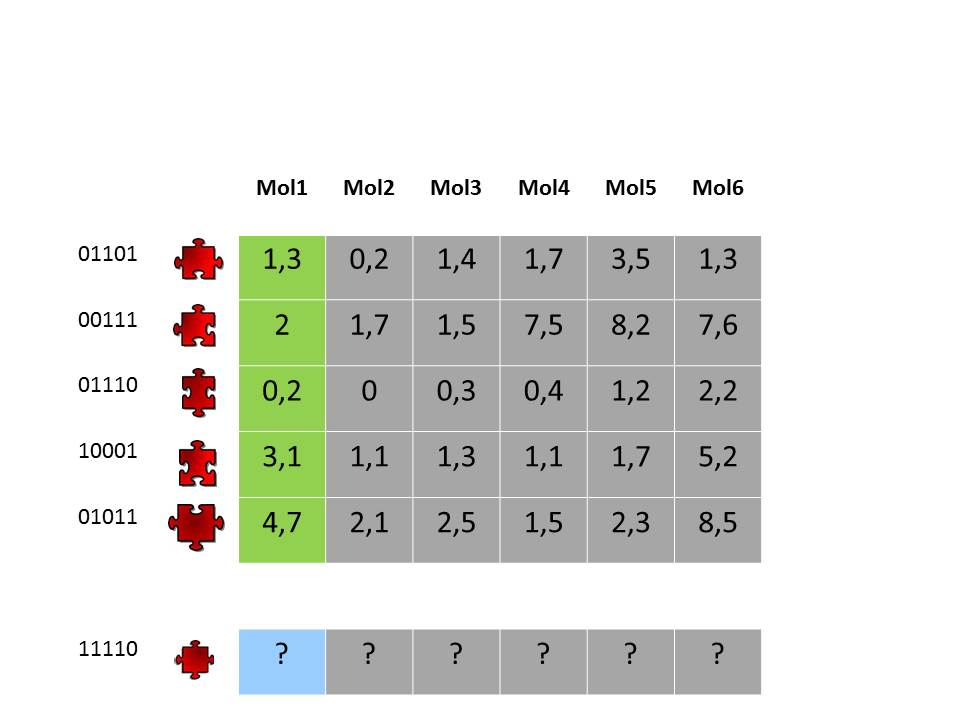
\includegraphics[width=0.3\textwidth,trim = 0 0 100 100,clip]{figure/Slide13}
		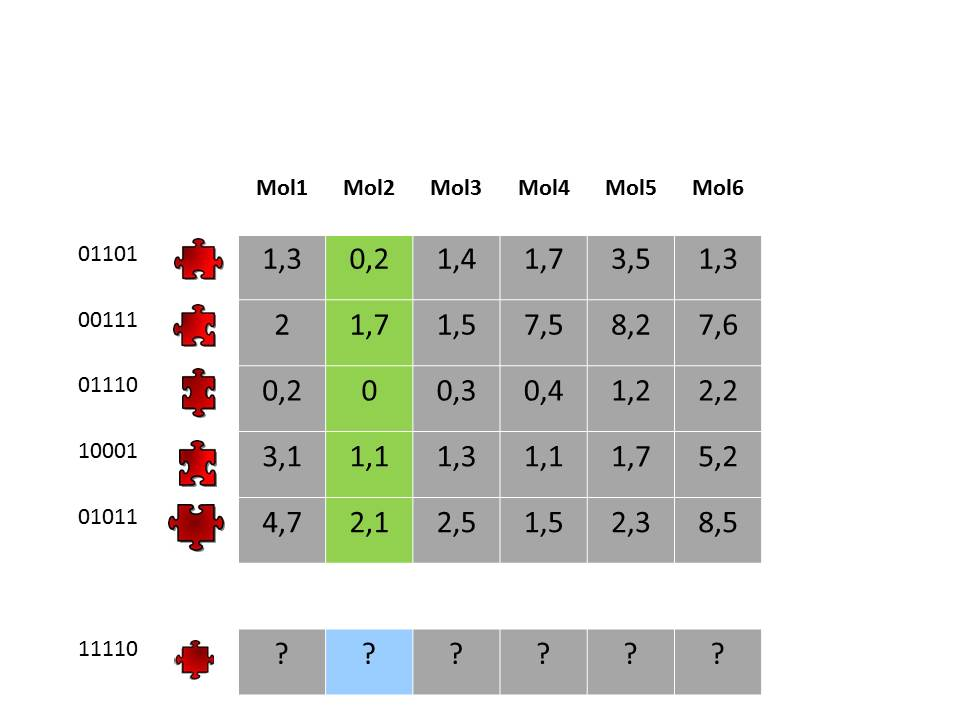
\includegraphics[width=0.3\textwidth,trim = 0 0 100 100,clip]{figure/Slide14} 
%		
		$\ldots$
%		
		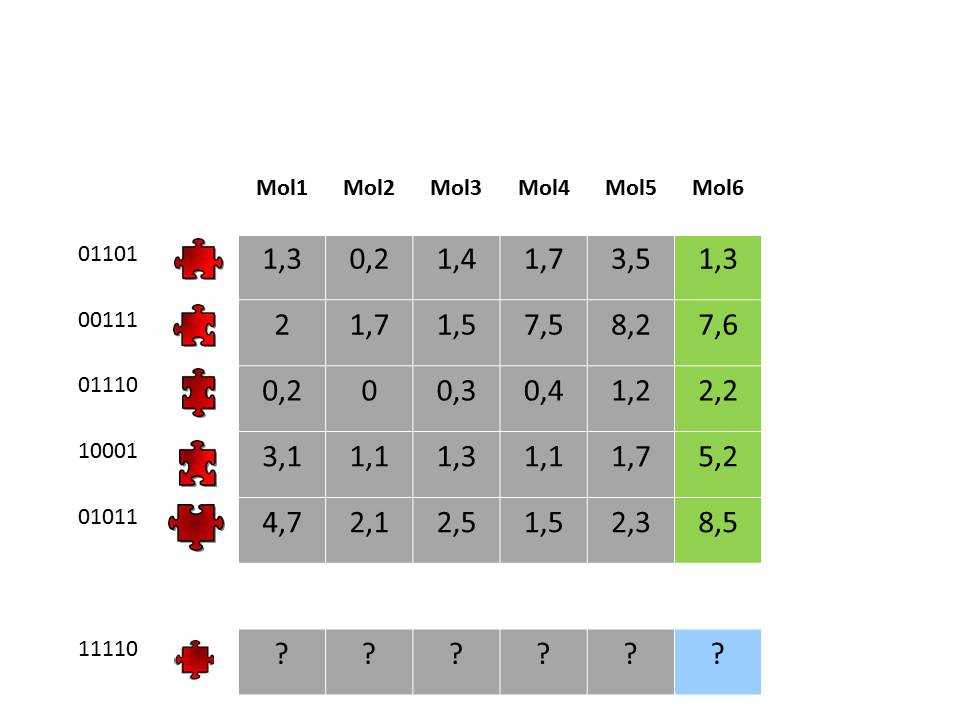
\includegraphics[width=0.3\textwidth,trim = 0 0 100 100,clip]{figure/Slide15}
	\end{figure}
%	
%
	\begin{itemize}
%		
		\item In multi-label classification this approach is also known as \emph{binary relevance learning.}
	%	
		\item The advantage of this approach is that it is quite easy to realize, as for single-target prediction we have a wealth of methods available.
	%
	\end{itemize}

\end{frame}

\begin{frame}{Independent Models}
%	
	\footnotesize
%	
	\begin{itemize}
%		
		\item 	We illustrate the typical approach by means of linear basis function model for the $j$-th target: 
		\begin{equation*}
			f_j(\xv) = \ba_j^\intercal \phi(\xv) \,,
			\label{eq:binrel}
		\end{equation*}
%	
		where $\ba_j$ is a target-specific parameter vector and $\phi$ some feature mapping.
%
		\item The parameter vectors are found by solving a (regularized) optimization problem: 
%		
		\begin{equation*}
			\label{eq:multiridge}
			\min_A \|Y - \Xmat A \|^2_F +  \sum_{j=1}^m \lambda_j \,\|\ba_j\|^2 \,,
		\end{equation*}
%	
		where $ \| B \|^2_F  = \sqrt{ \sum_{i=1}^n \sum_{j=1}^m B_{i,j}^2 } $ is the Frobenius norm for a matrix $B \in \R^{n \times m}$ and 
%		
		\begin{equation*}
			\label{eq:notation}
			\Xmat = \begin{bmatrix} \phi(\xv^{(1)})^\top \\ \vdots \\ \phi(\xv^{(n)})^\top \end{bmatrix} \qquad A = [\ba_1 \quad \cdots \quad \ba_m] \,.
		\end{equation*}
% 	$$Y: (n \times m) \qquad  X: (n \times p) \qquad A: (p \times m)$$
%
		\item The norm for regularizing the target-specific parameters can vary:
%		
			\begin{itemize} \footnotesize
%				
				\item L2-norm $\leadsto$ Multivariate Ridge Regression.
%				
				\item L1-norm $\leadsto$ Multivariate Lasso Regression.
%				
%				\item Combination of 
%				
			\end{itemize}
%	
	\end{itemize}
%
\end{frame}

\begin{frame}{Independent Models: Practical Performance}
%	
	The experimental results section of a typical MTP paper: 
%	
	\begin{center}
		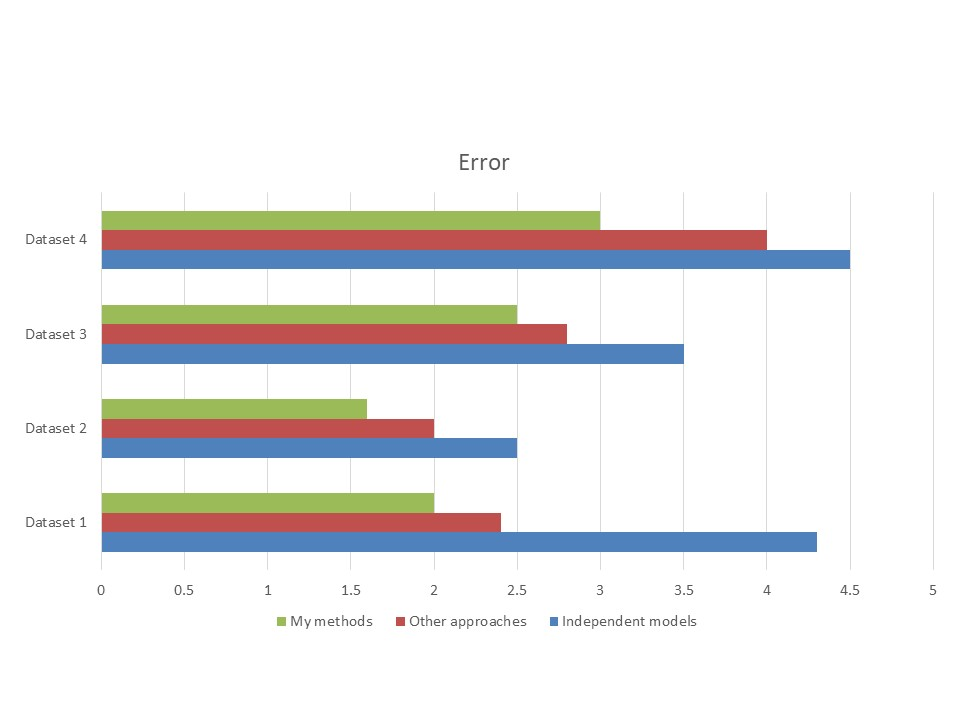
\includegraphics[scale=0.45, trim = 0 50 0 100,clip]{figure/barplots} \\
	\end{center}
%
	$\leadsto$ Independent models do not exploit target dependencies compared to more sophisticated methods, which seems to be a key for better performance in MTP problems.
%	
\end{frame}


\begin{frame}
	\frametitle{James-Stein estimation}
%	
	\footnotesize
%	
	\begin{itemize}
%		
		\item Consider a sample of a multivariate normal distribution $\yv \sim \normal(\thetab, \sigma^2\mathbf{I}),$ i.e., the components $y_1,\ldots,y_m$ of $\yv$ are independent of each other.
%		
		\begin{center}
			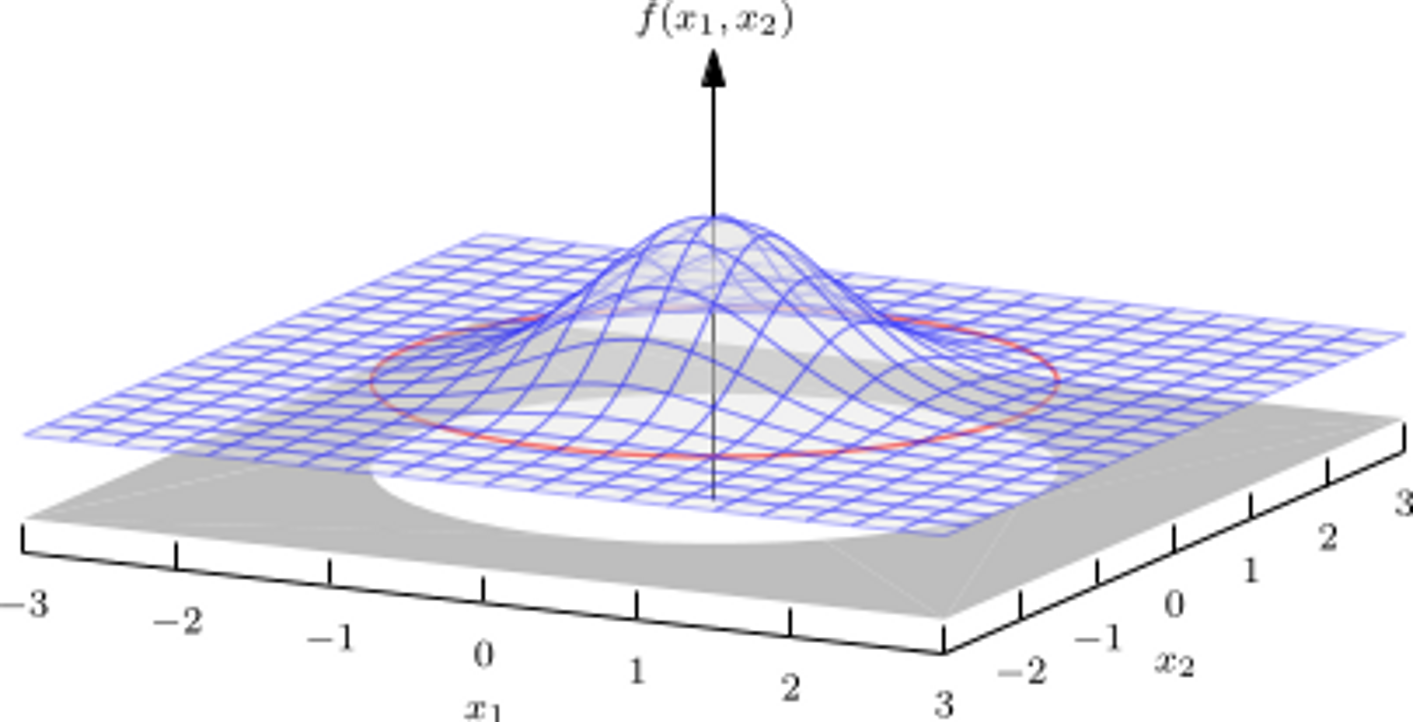
\includegraphics[width = 4cm]{figure/biva}
		\end{center}
%		
		\item What is the best estimator of the mean vector $\thetab$ w.r.t.\ mean-squared error (MSE): $\mathbb{E}[(\thetab - \thetabh)^2]?$  
%		
		\item The single-observation maximum likelihood estimator (which is also the least-squares estimate in this case) is $\thetabh^{\mathrm{ML}} = \yv.$  
%		
		\item The James-Stein estimator [James \& Stein (1961)]:
%		Estimation with quadratic loss 
		$$
		\thetabh^{\mathrm{JS}} = \left (1 - \frac{(m-2)\sigma^2}{\|\yv\|^2_2} \right )\yv
		$$
		has a smaller MSE than the maximum likelihood estimator!
%		
		\item[$\leadsto$] Improvements over independent predictions can be achieved even for problems without any statistical dependence between the targets!
%
		\item Explanation: The variance is reduced by introducing a bias.
%		
%
	\end{itemize}
	
\end{frame}




\begin{frame}
	\frametitle{James-Stein estimation}
	
	\footnotesize
	\begin{itemize}
		%\item Similar principle as many target regularization methods.
		
		\item Works best when the norm of the mean vector is close to zero:\\
		\begin{center}
			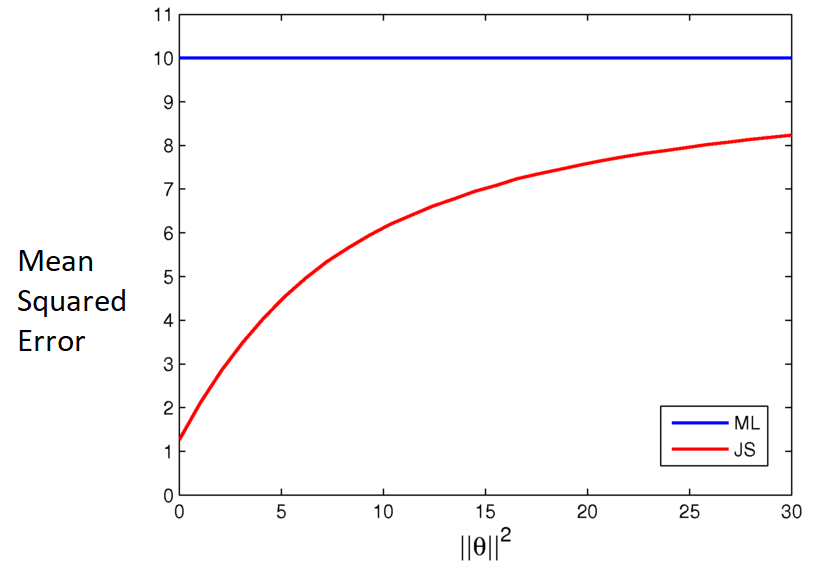
\includegraphics[width=5cm]{figure/JS}
		\end{center}  
		\item Regularization towards other directions, say $\bm{v}$, is also possible:
		$$
		\thetabh^{\mathrm{JS}}(\bm{v}) = \left (1 - \frac{(m-2)\sigma^2}{\|\yv - \bm{v}\|^2} \right )(\yv - \bm{v}) + \bm{v}
		$$
		\item Only outperforms the maximum likelihood estimator w.r.t.\ the sum of squared errors over all components, and only when $m \geq 3.$
		\item The result can be generalized to the case with $n$ iid observations of $\normal(\thetab, \sigma^2\mathbf{I})$ as well as for the case of iid samples of $\normal(\thetab, \bm{\Sigma})$ for a general covariance matrix $\bm{\Sigma}.$
%		\item Take-away message: 
	\end{itemize}
\end{frame}

\section{Similarity-enforcing methods}

\begin{frame}[t]
	\frametitle{Mean-regularized multi-task learning}
	
	\vspace{0.2cm}
	\begin{columns}
		\column{5cm}
		\footnotesize{
			\begin{itemize} 
%				
				\item \emph{Idea}: The models for the different targets should behave similar. How?
%				One can enforce similarity of the parametrizations of the models for the different targets.
%				
				\item \emph{Simple solution}: The parameters of these models should have similar values.
%				
				\item \emph{Approach}: Bias the parameter vectors towards their overall mean vector:
					\vspace{0.2cm}
				\begin{equation*}
					\label{eq:meanreg}
					\min_A \|Y - \Xmat A \|^2_F + \lambda \sum\nolimits_{j=1}^m \|\ba_j - \frac{1}{m} \sum\nolimits_{j'=1}^m \ba_{j'} \|^2 \, ,
				\end{equation*}
%				
				\item \emph{Disadvantage}: The assumption of all target models being similar might be invalid for many applications. \lz
			\end{itemize}
		}
		\column{4.5cm}
		
		\begin{tikzpicture}[
			level 1 concept/.append style={font=\sf, level distance = 21mm},
			level 2 concept/.append style={font=\sf, level distance = 21mm},
			every node/.append style={scale=0.5}]
			
			\path[mindmap, concept color=black,text=white]
			
			node[concept] {Mean}
			child[grow = 90, concept color=green!50!black] { node[concept] {Target 1}}
			child[grow = 180,concept color=blue] { node[concept] {Target 2}}
			child[grow = 270,concept color=red] { node[concept] {Target 3} }
			child[grow = 360,concept color=orange] { node[concept] {Target 4} };   
		\end{tikzpicture}
%	
	\end{columns}

{\tiny Evgeniou and Pontil, Regularized multi--task learning, KDD 2004}
\end{frame}


%\begin{frame}{Joint feature selection}
%	\small
%\begin{itemize}
%%	
%\item Enforce that the same features are selected for different targets:
%$$
%\min_A \|Y - XA \|^2_F +  \sum_{i=1}^p \lambda_j \|\ba^{(i)} \|^2  
%$$   
%%
%\item The vectors $\ba^{(i)}$ now represent the columns of matrix $A^T$:
%%
%\end{itemize}
%\begin{center}
%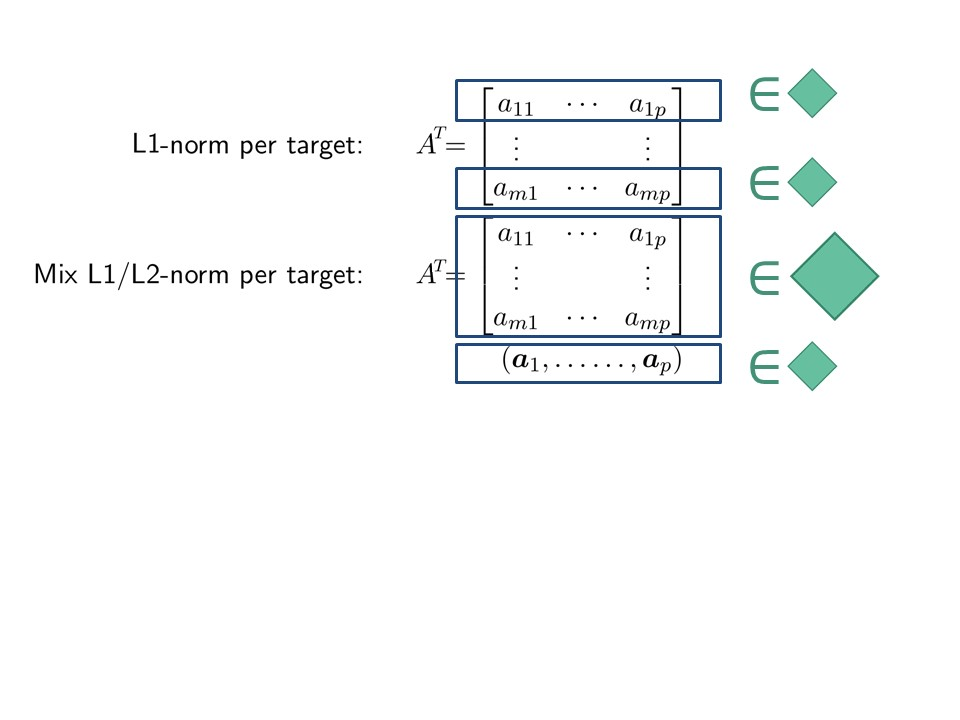
\includegraphics[width=0.9\textwidth,trim = 0 240 30 50,clip]{figure/Dia21}
%\end{center}
%%
%\begin{itemize}
%	%	
%	\item Using L1-norm or a combination of L1- and L2-norm can lead to sparsity.
%%	
%\end{itemize}
%%
%	{\tiny Obozinski et al., Joint covariate selection and joint subspace selection for multiple classification problems. Statistics and Computing 2010.}
%\end{frame}


\begin{frame}
	\frametitle{Stacking (Stacked generalization)}
	
	\begin{itemize}
%		
		\item Originally introduced as a general ensemble learning or blending technique.
%		
		\item Level 1 learners: apply a series of ML methods on the same dataset (or, one ML method on bootstrap samples of the dataset)
		\item Level 2 learner: apply an ML method to a new dataset consisting of the predictions obtaining at Level 1 
	\end{itemize}
	
	\begin{center}
		\def\layersep{1.25cm}
		\begin{tikzpicture}[shorten >=1pt,->,draw=black!50, node distance=\layersep]
			\tikzstyle{every pin edge}=[<-,shorten <=1pt]
			\tikzstyle{neuron}=[circle,fill=black!25,minimum size=17pt,inner sep=0pt]
			\tikzstyle{input neuron}=[neuron, fill=green!50];
			\tikzstyle{output neuron}=[neuron, fill=red!50];
			\tikzstyle{hidden neuron}=[neuron, fill=blue!50];
			\tikzstyle{annot} = [text width=4em, text centered]
			
			% Draw the input layer nodes
			\foreach \name / \y in {1,...,4}
			% This is the same as writing \foreach \name / \y in {1/1,2/2,3/3,4/4}
			\node[input neuron] (I-\name) at (\y, 0) {$f_\y$};
			
			% Draw the hidden layer nodes
			\foreach \name / \y in {1}
			% \path%[yshift=0.5cm]
			\node[hidden neuron] (H-\name) at (2.5, \layersep) {$h_\y$};
			
			
			% % Draw the output layer node
			\node[output neuron] (I) at (2.5, -\layersep) {$\xv$};
			%%
			%%    % Connect every node in the input layer with every node in the
			%%    % hidden layer.
			\foreach \source in {1,...,4}
			\foreach \dest in {1}
			\path (I-\source) edge (H-\dest);
			%%
			%    % Connect every node in the hidden layer with the output layer
			\foreach \source in {1,...,4}
			\path (I) edge (I-\source);
			%
			% Annotate the layers
			\node[annot,left of=H-1, node distance=3cm] (hl) {Level 2}; 
			\node[annot,below of=hl, node distance=\layersep] {Level 1};
			%%    \node[annot,right of=hl] {Output layer};
		\end{tikzpicture}
	\end{center}
	{\tiny Wolpert, Stacked generalization. Neural Networks 1992.}
	%D. Wolpert, Stacked Generalization, Machine Learning, 1992
\end{frame}

\begin{frame}
	\frametitle{Stacking applied to MTP }
	\footnotesize
	\begin{columns}
		\begin{column}{4.5cm}
			\begin{itemize}
%				
				\item Level 1 learners: learn a model for every target independently 
%				
				\item   [$\leadsto$] $f_1,\ldots,f_m$
%				
				\item Level 2 learner: learn again a model for every target independently, using the predictions of the first step as features
%				
				\item   [$\leadsto$] $f(\xv) = h(f_1(\xv),\ldots,f_m(\xv))$ \\
				Or alternatively: $f(\xv) = h(f_1(\xv),\ldots,f_m(\xv),\xv)$  \\
%				
%				 
			\end{itemize}
		\end{column}
		
		\begin{column}{5cm}
			\def\layersep{2cm}
			\begin{tikzpicture}[shorten >=1pt,->,draw=black!50, node distance=\layersep]
				\tikzstyle{every pin edge}=[<-,shorten <=1pt]
				\tikzstyle{neuron}=[circle,fill=black!25,minimum size=17pt,inner sep=0pt]
				\tikzstyle{input neuron}=[neuron, fill=green!50];
				\tikzstyle{output neuron}=[neuron, fill=red!50];
				\tikzstyle{hidden neuron}=[neuron, fill=blue!50];
				\tikzstyle{annot} = [text width=4em, text centered]
				
				% Draw the input layer nodes
				\foreach \name / \y in {1,...,4}
				% This is the same as writing \foreach \name / \y in {1/1,2/2,3/3,4/4}
				\node[input neuron] (I-\name) at (\y, 0) {$f_\y$};
				
				% Draw the hidden layer nodes
				\foreach \name / \y in {1,...,4}
				% \path%[yshift=0.5cm]
				\node[hidden neuron] (H-\name) at (\y, \layersep) {$h_\y$};
				
				
				% % Draw the output layer node
				\node[output neuron] (I) at (2.5, -\layersep) {$\xv$};
				%%
				%%    % Connect every node in the input layer with every node in the
				%%    % hidden layer.
				\foreach \source in {1,...,4}
				\foreach \dest in {1,...,4}
				\path (I-\source) edge (H-\dest);
				%%
				%    % Connect every node in the hidden layer with the output layer
				\foreach \source in {1,...,4}
				\path (I) edge (I-\source);
				%
				% Annotate the layers
				\node[annot,left of=H-1, node distance=1cm] (hl) {Level 2}; 
				\node[annot,left of=I-1, node distance=1cm] {Level 1};
				%%    \node[annot,right of=hl] {Output layer};
			\end{tikzpicture}
		\end{column}
	\end{columns}
%
	\begin{itemize}
%		\item 
		\item Advantages: Easy to implement and general (usable with any level-1 learner). 
		\item Has been shown to avoid overfitting in multivariate regression.
		\item If level 2 learner uses regularization $\leadsto$ models are forced to learn similar parameters for different targets.  
	\end{itemize}
	% 
	{\tiny Cheng and H\"ullermeier, Combining Instance-based learning and Logistic Regression for Multi-Label classification, Machine Learning, 2009.}
	
\end{frame}

\begin{frame}{Enforcing similarity in (Deep) Neural Networks}
	\small
	\begin{center}
		Commonly-used architecture: weight sharing in the final layer with $m$ nodes, i.e., weight sharing among the targets \\
		\vspace{0.2cm}
		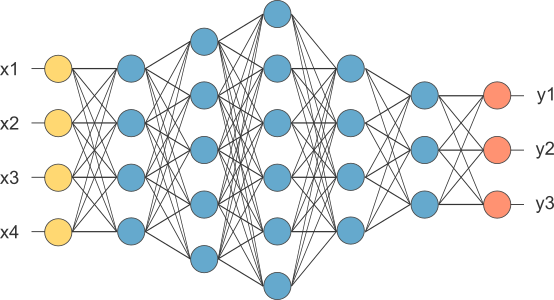
\includegraphics[scale=0.4]{figure/weightsharing}
	\end{center}

{\tiny Caruana, Multitask learning: A knowledge-based source of inductive bias. Machine	Learning 1997.}
\end{frame}


\section{Similarity-exploiting methods}


\begin{frame}{Kronecker kernel ridge regression}
	\footnotesize
	\begin{itemize}
%		
	\item In the case of multi-target prediction with target features one typically uses kernel methods for learning.
%		
	\item In particular, one considers the following pairwise model representation in the primal: 
		\begin{equation*}
			\label{eq:pairwise}
			f(\xv,\tv) = \bm\omega^\top \left(\phi(\xv) \otimes \psi(\tv) \right) ,
		\end{equation*}
%	
	where $\phi$ is some feature map for the features and $\psi$ is a feature map for the target (features) and $\otimes$ is the Kronecker product.
%
	\item This leads to the Kronecker product pairwise kernel in the dual:
%	
	\begin{eqnarray*} 
		f(\xv,\tv)= \sum_{(\xv',\tv') \in \D} \alpha_{(\xv',\tv')}  \cdot  k(\xv,\xv') \cdot g(\tv,\tv')  = \sum_{(\xv',\tv') \in \D} \alpha_{(\xv',\tv')} \Gamma((\xv,\tv),(\xv',\tv')),
	\end{eqnarray*}
%
	where $k$ is the kernel for the feature map $\phi,$  $g$ the kernel for the feature map $\psi$  and $\alpha_{(\xv',\tv')}$ are the dual parameters, which can be found by least-squares minimization:
%	 
	$$ \min_{\bm{\alpha}} \, ||\bm{\Gamma}\bm{\alpha} -\bm{z} ||^2_2 +\lambda\bm{\alpha }^\top \bm{\Gamma}\bm{\alpha}, $$
%	
	where $\bm{z} = \mathrm{vec}{(Y)}.$
%
%	\item Idea: Model the joint kernel as a product of an instance kernel $k(\cdot,\cdot)$ and a target kernel $g(\cdot,\cdot)$: 
%		$$\Gamma((\xv,\tv),(\xv',\tv')) = k(\xv,\xv') \cdot g(\tv,\tv')$$
%
	\item This approach is commonly used in the zero-shot learning framework.

%
\end{itemize}
%	
	{\tiny Stock et al., A comparative study of pairwise learning methods based on kernel ridge regression, Neural Computation 2018.}
%	
\end{frame}



\begin{frame}{Exploiting relations in regularization terms}
	\footnotesize
%
	\begin{center}
		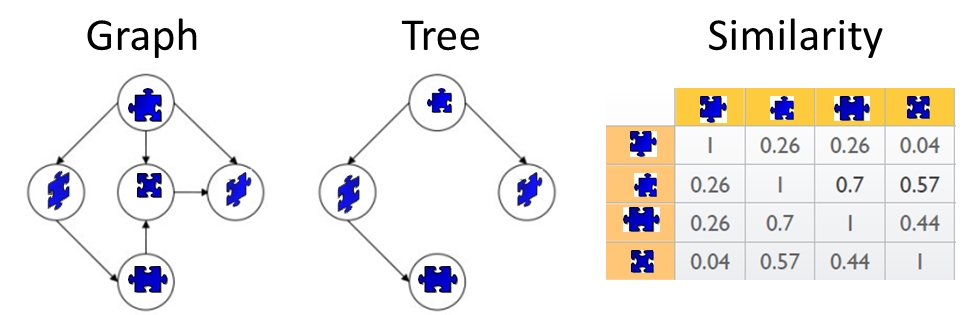
\includegraphics[width=\textwidth]{figure/targetrelations}
	\end{center} 
%	
	\begin{itemize}
%		
		\item 	Graph-based regularization is an approach that can be applied to the tree types of relations in the targets: 
		%
		\begin{equation*}
			\min_A \|Y - XA \|^2_F + \lambda \sum_{j=1}^m \sum_{j' \in \mathcal{N}(j)} \|\ba_j - \ \ba_{j'}\|^2,
		\end{equation*}
		%
		where $\mathcal{N}(j)$ is the set of targets that are related to target $j.$
%		
		\item Can also be used in a weighted version taking the similarities (or correlations) into account.
%		
	\end{itemize}
	
%
	{\tiny Gopal and Yang, Recursive regularization for large-scale classification with hierarchical and graphical dependencies, KDD 2013.}
\end{frame}

\begin{frame}{Hierarchical multi-label classification}
	\small
	\vspace{-0.2cm}
	\begin{center}
		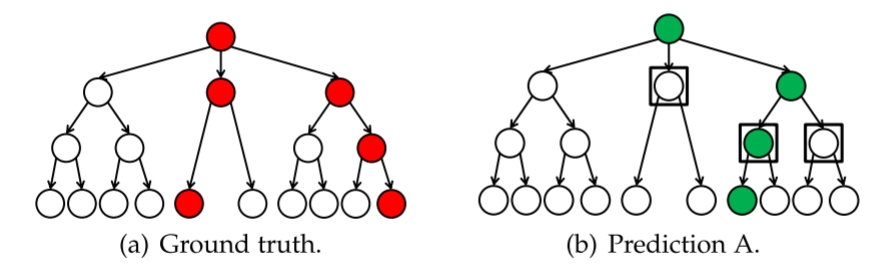
\includegraphics[width=\textwidth]{figure/hloss}
	\end{center}
	
	\vspace{-0.2cm}
	\begin{minipage}{0.75\textwidth}   
	\begin{itemize}
%		
		\item %	
		In addition to performance gains in general, hierarchies can also be used to define specific loss functions, such as the Hierarchy-loss: 
		%	
		$$\ell_{Hier}(\yv,\hat{\yv}) = \sum_{j: y_j \neq \hat{y_j}} c_j \, \mathds{1}_{ [\textit{anc}(y_j) = \textit{anc}(\hat{y}_j)]  },$$
		%	
		where $c_j$ are costs depending on the depth of node $j.$
		%	
%		
	\end{itemize}
\end{minipage}
\begin{minipage}{0.2\textwidth}    
	\begin{center}
		%    	
		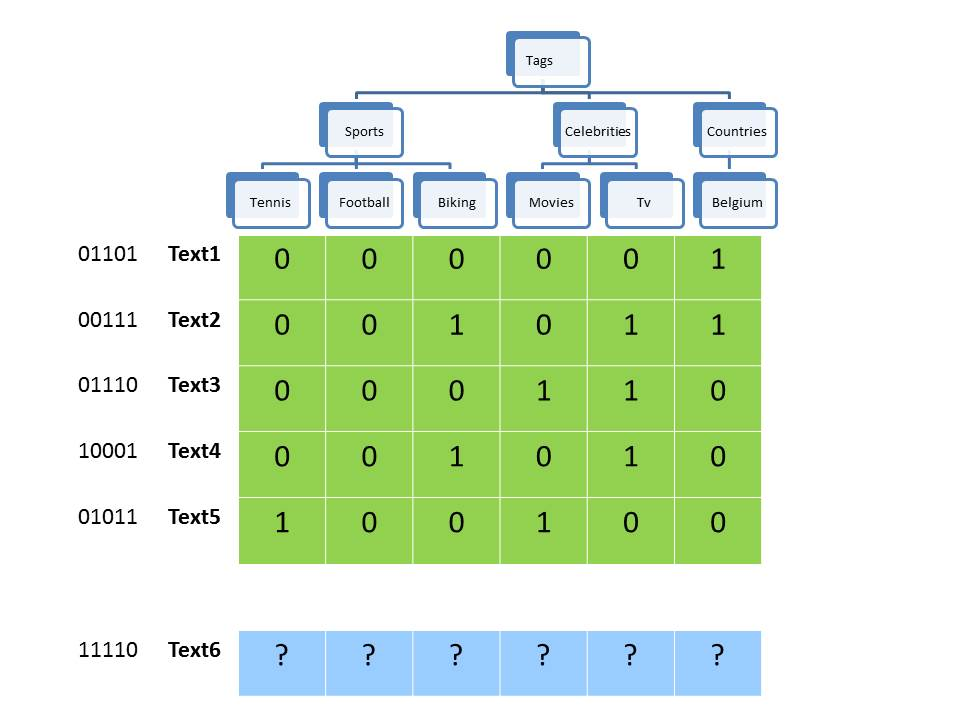
\includegraphics[width=0.99\textwidth,trim = 0 0 100 20,clip]{figure/Slide5}
		%    	
	\end{center}
\end{minipage}
\begin{itemize}
%	
	\item This is rather common in multi-label classification problems.
%	
\end{itemize}

	{\tiny Bi and Kwok, Bayes-optimal hierarchical multi-label classification, IEEE Transactions on Knowledge and Data Engineering, 2014.}
%
\end{frame}



\section{Similarity-constructing methods}




\begin{frame}
	\frametitle{Probabilistic classifier chains}
	
	\begin{itemize}
		\item Estimate the \alert{joint} conditional distribution $\P(\yv ~|~  \xv)$. 
		\item For optimizing the \alert{subset 0/1} loss:  $$ \ell_{0/1}(\yv, \hat{y}) = \mathds{1}_{[\yv \ne \hat{y}]}$$
		\item Repeatedly apply the \emph{product rule} of probability:
		$$
		\P(\yv ~|~ \xv) = \prod_{j=1}^{m} \P(y_j ~|~ \xv, y_1, \ldots,y_{j-1}) \, .
		$$
		\item  Learning relies on constructing \alert{probabilistic classifiers} for estimating 
		$$
		\P( y_i|\xv, y_1, \ldots,y_{j-1}) \,,
		$$
		{independently} for each $j = 1, \ldots, m$. 
		%\item One can use scoring functions $f_i(\xv^\prime,y_i)$ and use logistic transformation.
		%\item By using the linear models, the overall scoring function takes the form:
		%$$
		%f(\xv,\yv) = \sum_{i=1}^m f_i(\xv, y_i) + \sum_{y_k,y_l} \! f_{k,l}(y_k,y_l) 
		%$$
	\end{itemize}
\end{frame}

\begin{frame}[fragile]
	\frametitle{Probabilistic classifier chains}
	\begin{itemize}
		\item Inference relies on exploiting a probability tree:
	\end{itemize}
	\vspace{0.1cm}
	\begin{center}
		\begin{tikzpicture}[scale = 0.85,every node/.style={scale=0.85},
			regnode/.style={circle,draw,minimum width=1.5ex,inner sep=0pt},
			leaf/.style={circle,fill=black,draw,minimum width=1.5ex,inner sep=0pt},
			pleaf/.style={rectangle,rounded corners=1ex,draw,font=\scriptsize,inner sep=3pt,line width=1pt},
			pnode/.style={rectangle,rounded corners=1ex,draw,font=\scriptsize,inner sep=3pt},
			rootnode/.style={rectangle,rounded corners=1ex,draw,font=\small,inner sep=4pt},
			level/.style={sibling distance=16em/#1, level distance=12ex}
			]
			\node (z) [rootnode] {$\xv$}
			child {node (a) [pnode] {$P(y_1=0 ~|~ \xv)=0.4$} 
				child {node [label=below:{\scriptsize \thickmuskip=0mu $P(\yv=(0,0)~|~ \xv)=0$}] (b) [pleaf] {\thickmuskip=-1.5mu $P(y_2=0 ~|~ y_1=0, \xv)=0.0$} edge from parent node[above left]{$y_2=0$}}
				child {node [label=below:{\color{blue} \scriptsize \thickmuskip=0mu $P(\yv=(0,1) ~|~ x)=0.4$}] (g) [pleaf] {\thickmuskip=-1.5mu $P(y_2=1 ~|~ y_1=0, \xv)=1.0$} edge from parent node[above right]{$y_2=1$}}
				edge from parent node[above left]{$y_1=0$}
			}
			child {node (j) [pnode] {$P(y_1=1 ~|~ \xv)=0.6$}
				child {node [label=below:{\scriptsize \thickmuskip=0mu $P(\yv=(1,0) ~|~ \xv)=0.24$}] (k) [pleaf] {\thickmuskip=-1.5mu $P(y_2=0 ~|~ y_1=1, \xv)=0.4$} edge from parent node[above left]{$y_2=0$}}
				child {node [label=below:{\color{red} \scriptsize \thickmuskip=0mu $P(\yv=(1,1) ~|~ \xv)=0.36$}] (l) [pleaf] {\thickmuskip=-1.5mu $P(y_2=1 ~|~ y_1=1, \xv)=0.6$}
					{
						child [grow=right] {node (s) {} edge from parent[draw=none]
							child [grow=up] {node (t) {} edge from parent[draw=none]
								child [grow=up] {node (u) {} edge from parent[draw=none]}
							}
						}
					}
					edge from parent node[above right]{$y_2=1$}
				}
				edge from parent node[above right]{$y_1=1$}
			};
			
			%\path (s) -- (t) node [midway] {$\lambda_{2}$};
			%\path (t) -- (u) node [midway] {$\lambda_{1}$};
		\end{tikzpicture}
	\end{center}
	
	\vspace{0.1cm}
	\begin{itemize}\small
		\item For subset 0/1 loss one needs to find $
		\fbayes(\xv) = \argmax_{\yv \in \Yspace^m} \P(\yv ~|~ \xv)
		$.
		\item Greedy and approximate search techniques with guarantees exist.
%		\footnote{Kumar et al., Beam search algorithms for multilabel
%	learning, Machine Learning 2013}
		\item Other losses: compute the prediction on a sample from $\P(\yv ~|~  \xv).$
%		\footnote}
		%\item[]
	\end{itemize}
{\tiny Dembczynski et al., An analysis of chaining in multi-label classification, ECAI 2012.}
	
\end{frame}



\begin{frame}{Low-rank approximation}
	
	\begin{center}
		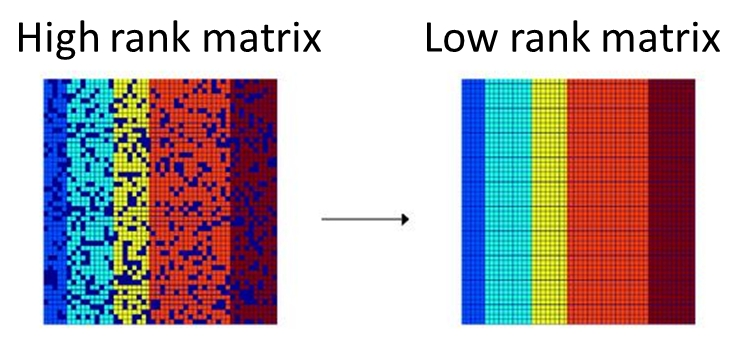
\includegraphics[width=9cm]{figure/lowrank}
	\end{center}

	\begin{itemize}
%		
		\item Low rank materializes the idea that some structure is shared across different targets.
%
		\item 	Typically perform a low-rank approximation of the parameter matrix:
		$$\min_A \|Y - \Xmat A \|^2_F + \lambda \, \mathrm{rank}(A)$$
%		
	\end{itemize}
	{\tiny Chen et al., A convex formulation for learning shared structures from
	multiple tasks, ICML 2009.}
\end{frame}



%%%%%%%%%%%%%%%%%%%%%%%%%%%%%%%%%%%%%%%%%%%%%%%%%%%%%%%%%%%%%%%%%%%%%%%%%%%%%% 
%%%%%%%%%%%%%%%%%%%%%%%%%%%%%%%%%%%%%%%%%%%%%%%%%%%%%%%%%%%%%%%%%%%%%%%%%%%%%%  

%%%%%%%%%%%%%%%%%%%%%%%%%%%%%%%%%%%%%%%%%%%%%%%%%%%%%%%%%%%%%%%%%%%%%%%%%%%%%% 
%%%%%%%%%%%%%%%%%%%%%%%%%%%%%%%%%%%%%%%%%%%%%%%%%%%%%%%%%%%%%%%%%%%%%%%%%%%%%% 
\frame{
	\frametitle{Low-rank approximation}
	
	
	
	\begin{itemize}
		\item $A$: parameter matrix of dimensionality $p \times m$ 
		\item $p$: the number of features
		\item $m$: the number of targets
		\item Assume a low-rank structure of $A$:\\
%		
		$ \qquad  \qquad\qquad \quad  U  \quad \times \qquad  V \qquad \quad  =  \qquad  A$
		\begin{center}
%					
			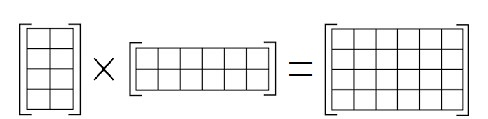
\includegraphics[width=0.6\textwidth,trim = 0 0 0 0,clip]{figure/uv_decomp}
%
		\end{center}
		
		\item We can write $A=UV$ and $A \xv = UV \xv$
		\item $V$ is a $p \times \hat{m}$ matrix
		\item  $U$ is an $\hat{m} \times m$ matrix
		
		\item $\hat{m}$ is the rank of $A$
		
	\end{itemize}
	
}

\begin{frame}{Low-rank approximation: Overview of methods}
	
	\begin{itemize}
		\item Popular for multi-output regression, multi-task learning and multi-label classification.
		\item Linear as well as nonlinear methods.
		\item Algorithms: 
		\begin{itemize}
			\item Principal component analysis, Canonical correlation analysis, Partial least squares.
			\item Singular value decomposition, Alternating structure optimization.
			\item Compressed sensing, Output codes, Landmark labels, Bloom filters, Auto-encoders.
		\end{itemize}
	\end{itemize}
%   \footnote{Weston et al., Kernel dependency estimation, NIPS 2002}
% 	\footnote{Multi-label prediction via sparse infinite CCA, NIPS 2009}
%\footnote{Tai and Lin, Multilabel classification with principal label space transformation, Neural Computation 2012}
%  	\footnote{Zhou et al., Clustered Multi-Task Learning Via Alternating Structure Optimization, NIPS 2011}
%	\footnote{Hsu et al., Multi-label prediction via compressed sensing. NIPS 2009}
%	\footnote{Zhang and Schneider, Multi-label Output Codes using Canonical Correlation Analysis, UAI 2011}
%	\footnote{Balasubramanian and Lebanon, The landmark selection method for multiple output
%	prediction, ICML 2012}
%	\footnote{Ciss\'e et al., Robust bloom filters for large multilabel
%	classification tasks, NIPS 2013}
% 	\footnote{Wicker et al., A nonlinear label compression and transformation
%	method for multi-label classification using autoencoders, PAKDD 2016}
	\vspace{0.3cm}
\end{frame}


%
\endlecture
\end{document}
